\chapter{Considerações Finais} \label{cap:consideracoes_finais}

Este trabalho apresentou a proposta de uma API para uma plataforma de
participação social e sua adaptação para o contexto de violência contra a mulher.

% analisar a ideia do ``Empurrando Juntos''. A partir dessa etapa, foi possível entender
% o seu atual funcionamento, que consiste apenas pelo módulo de clusterização, e por consequência identificar as necessidades da plataforma.
% Além disso, nessa etapa foi realizado um levantamento das aplicações existentes na temática de violência contra a mulher com o intuito de 
% entender suas contribuições e lacunas para este contexto.
% 
% A partir das informações obtidas na etapa de diagnóstico, foi realizada a segunda etapa do trabalho, na qual as necessidades identificadas
% foram convertidas em uma proposta de solução.

Nesta primeira fase do trabalho, foram realizadas as etapas de ``Diagnóstico'' e ``Definição da proposta'', cuja realização foi descrita nos capítulos anteriores. 
Por fim, também foi realizada a etapa de ``Planejamento'', com a realização de um cronograma que pode ser visto na Figura \ref{fig:planejamento}.


% \begin{table}[h!]
% \centering
% \caption{Planejamento do trabalho}
% \label{tab:planejamento}
% \begin{tabular}{@{}cl@{}}
% \toprule
% \multicolumn{2}{c}{\textbf{Metas}}                                                                                                                         \\ \midrule
% \multirow{3}{*}{Iteração 1}           & Estabelecimento da arquitetura                                                                                     \\
%                                       & Implementação da feature de Gerenciamento de Usuário                                                               \\
%                                       & Autenticação                                                                                                       \\ \midrule
% \multirow{2}{*}{Iteração 2}           & Implementação da feature de Gerenciamento de Conversa                                                              \\
%                                       & Implementação da feature de Gerenciamento de Comentário                                                            \\ \midrule
% \multirow{2}{*}{Iteração 3}           & Implementação da feature de Agrupamento de usuários                                                                \\
%                                       & Definição dinâmica da semântica dos votos                                                                          \\ \midrule
% \multirow{2}{*}{Aplicação em um caso} & \begin{tabular}[c]{@{}l@{}}Estudo da adaptação da API para a temática de violência \\ contra a mulher\end{tabular} \\
%                                       & Construção de um exemplo de uso da API                                                                             \\ \bottomrule
% \end{tabular}
% \end{table}

\begin{figure}[ht!]
\centering
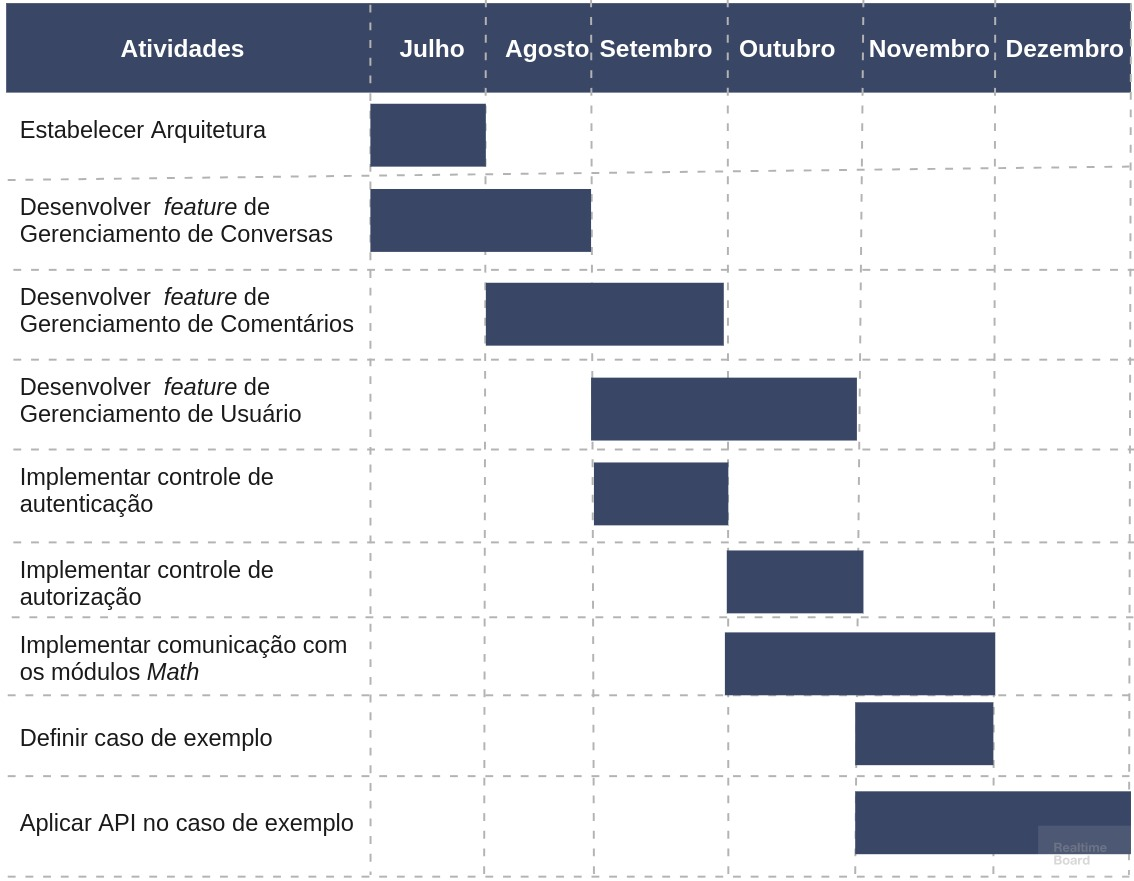
\includegraphics[scale=0.45]{figuras/cronograma.jpg}
\caption{Cronograma de execução do trabalho}
\label{fig:planejamento}
\end{figure}

No cronograma apresentado foram contempladas as duas últimas etapas do trabalho, conforme definido na Introdução. Além disso,
no final deste trabalho, as duas primeiras atividades listadas já foram iniciadas. Assim, a arquitetura da API e uma parte da \textit{feature}
de Gerenciamento de Conversas foi implementada.

No final da execução das demais etapas do trabalho é esperado uma API REST que seja capaz de fornecer um serviço de participação com conversas, comentários
e votos que agrupe pessoas a partir de suas opiniões. A criação da API contribuirá para a formação da plataforma ``Empurrando Juntos'' 
através da implementação da parte servidor da arquitetura definida.

No contexto social, o objetivo é que a API possa contribuir no apoio à mulheres vítimas de violência dentro das plataformas existentes, através
da promoção de discussões mais efetivas, da possibilidade de promover políticas públicas e da criação de uma rede de apoio entre mulheres que passam ou passaram por essa situação.
